\documentclass[11pt,letterpaper]{article}
\usepackage[T1]{fontenc}
\usepackage{lmodern}
\usepackage[margin=0.88in,top=0.82in,bottom=0.86in,headheight=15pt]{geometry}
\usepackage{amsmath,amssymb,amsthm,mathtools}
\usepackage{booktabs,array,tabularx,longtable}
\usepackage{graphicx,xcolor,microtype,enumitem,fancyhdr,needspace}
\usepackage{xurl,hyperref}
\definecolor{navy}{HTML}{17384B}
\definecolor{teal}{HTML}{167D8D}
\definecolor{muted}{HTML}{536675}
\hypersetup{colorlinks=true,linkcolor=teal,urlcolor=teal,citecolor=teal,
pdftitle={Beyond Dirichlet GRH: certified graph optima and quantitative local transfers},
pdfauthor={Research prepared for Vladimir Reshetnikov}}
\pagestyle{fancy}\fancyhf{}
\fancyhead[L]{\small\sffamily\color{navy}Beyond Dirichlet GRH}
\fancyhead[R]{\small\sffamily\color{muted}26 November 2026}
\fancyfoot[C]{\small\thepage}
\setlength{\parindent}{0pt}
\setlength{\parskip}{5pt plus 1pt minus 1pt}
\setlength{\emergencystretch}{2em}
\setlist{itemsep=3pt,topsep=5pt,leftmargin=1.5em}
\newtheorem{theorem}{Theorem}[section]
\newtheorem{lemma}[theorem]{Lemma}
\newtheorem{proposition}[theorem]{Proposition}
\newtheorem{corollary}[theorem]{Corollary}
\theoremstyle{definition}\newtheorem{definition}[theorem]{Definition}
\newcommand{\Q}{\mathbb Q}
\newcommand{\Z}{\mathbb Z}
\newcommand{\R}{\mathbb R}
\newcommand{\F}{\mathbb F}
\newcommand{\C}{\mathbb C}
\newcommand{\cO}{\mathcal O}
\newcommand{\Sha}{\mathrm{Sha}}
\newcommand{\src}[2]{\href{https://github.com/lsernau/grh-lean/blob/72fead102f663d5c7a407964a13dc0cf9d977207/grh/src/#1}{#2}}
\newcommand{\code}[1]{{\small\texttt{\detokenize{#1}}}}
\begin{document}
\hypersetup{pageanchor=false}
\begin{titlepage}
\thispagestyle{empty}
{\sffamily\large\color{teal}RESEARCH REPORT \hfill 26 NOVEMBER 2026\par}
\vspace{1.1cm}
{\fontsize{28}{34}\selectfont\bfseries\color{navy}Beyond Dirichlet GRH\par}
\vspace{0.4cm}
{\Large Certified graph optima and quantitative local transfers\par}
\vspace{0.7cm}
{\large Prepared for Vladimir Reshetnikov\par}
\vspace{0.7cm}\hrule\vspace{0.6cm}

\textbf{Question.} Can methods occurring in
\href{https://github.com/lsernau/grh-lean}{\texttt{lsernau/grh-lean}}
resolve other mathematical questions, beyond familiar consequences of RH and
Dirichlet GRH, while building on the ProveIt incoming reports?

\textbf{Answer.} Yes at the level of transferable ingredients, with concrete
certified results. This report extends the previous signed-cycle analysis to
seven previously untreated sizes, including an exact global optimum and all
minimizers at fifty vertices. It proves an exact coefficient-valuation formula
for Lubin--Tate logarithms and repairs the computational baseline for a related
coefficient-depth problem. It also independently revalidates two substantial
results already present in the incoming collection.

The difficult arithmetic mechanism behind the GRH proof has a clear extension
program, but this work does not prove a new general Artin, automorphic,
Selmer-vanishing, or algebraic \(K\)-theory conjecture.

\vspace{0.3cm}
\begin{tabularx}{\linewidth}{@{}p{0.25\linewidth}X@{}}
\toprule
\textbf{Contribution} & \textbf{Result and evidence}\\
\midrule
New graph cases &
Exact optima for \(n=34,36,38,42,44,46,50\), with complete rational and integer
certificates. At \(50\), \(2.811568906156<\rho_{\min}<2.811568906157\).\\
New local theorem &
For \(q=p^f\), \(N=v_p(n)\), and \(1\le j\le p^N\),
\(v_p([X^{n+j(q-1)}]L(X)^n)=N-v_p(j)-j\).\\
Earlier results checked &
Corrected optimum for every \(C_{8m}(1,2)\), \(m\ge4\), and strict
natural-versus-upper density gaps for geometric-progression-free sets.\\
Audit boundary &
46 prior archives inventoried. Selected proofs and certificates reviewed.
Upstream Lean source inspected; its full kernel build was not repeated.\\
\bottomrule
\end{tabularx}

\vfill
{\small\color{muted}
Source snapshots: \texttt{grh-lean} \texttt{72fead102f66};
\texttt{ProveIt} \texttt{5cc267af75a6}.\par
New results are written proofs with exact executable certificates, not new Lean
formalizations. Novelty is relative to the inspected incoming corpus;
worldwide publication priority is not asserted.}
\end{titlepage}
\hypersetup{pageanchor=true}
\pagenumbering{roman}
\tableofcontents
\clearpage
\pagenumbering{arabic}

\section{Scope, evidence, and what has advanced}
\label{sec:scope}

The starting point is the theorem package as it is actually stated in the
repository. \src{Statements.lean}{\texttt{Statements.lean}} defines assertions
in Mathlib's own language, and \src{Main.lean}{\texttt{Main.lean}} exports five
theorems. These cover the Riemann hypothesis, a critical-line formulation for
the zeta function, and right-half-plane and critical-strip statements for
Dirichlet \(L\)-functions, including imprimitive characters and every positive
modulus. The pole exception for the principal character is explicit.
The package does not state GRH for arbitrary nonabelian Artin representations
or all automorphic \(L\)-functions \cite{Repo}.

This scope leaves concrete extension targets. It also prevents treating an
already-known consequence of the Dirichlet endpoint as a new transfer.
We distinguish three kinds of work:

\begin{enumerate}
\item \textbf{Endpoint consequences.} Results obtained simply by assuming RH
or Dirichlet GRH. These are outside the principal aim of this report.
\item \textbf{Transfers of the arithmetic mechanism.} A new statistic is encoded
by integral objects, amplified by lifts, and constrained by matching upper and
lower determinant bounds. These are the ambitious arithmetic directions.
\item \textbf{Transfers of ingredients.} A component such as a Schur complement,
finite Fourier orthogonality, or sharp coefficient divisibility is adapted to
a different problem. Such an adaptation can solve a real problem while using
tools older than the GRH proof itself.
\end{enumerate}

The graph and local-series results below belong to the third category.
The new mathematics is in the graph-specific exhaustive obstruction and
boundary conditions, and in the exact coefficient calculation and its
application. We do not credit the GRH repository with inventing the underlying
Schur-complement or Fourier identities.

\subsection{Pinned sources and verification levels}

The upstream revision is
\[
\texttt{72fead102f663d5c7a407964a13dc0cf9d977207}.
\]
The ProveIt incoming snapshot is
\[
\texttt{5cc267af75a635199ac5d93a7d49cbce521daefc}.
\]
It contains 46 GRH-related ZIP archives. The archive names, SHA-256 hashes,
internal TeX inventories, and selected source-file hashes are included.
Inventorying an archive is not an endorsement of all its claims.

The source pins Lean \(4.35.0\) and Mathlib revision
\texttt{56a005855ea17e0b0958f73ec801ae140b0a1679}.
Upstream reports kernel builds, the axiom list
\code{propext}, \code{Classical.choice}, \code{Quot.sound}, independent
export checkers, and Comparator checks \cite{Repo}. Here, neither Lean nor
Lake was available, so these upstream checks were not repeated.

A reproducible lexical audit removed nested comments and strings and found no
\code{sorry}, \code{admit}, \code{axiom}, \code{unsafe},
\code{implemented_by}, or \code{native_decide} token in either \code{src}
tree. The simple import traversal reaches the 803 readable source modules
and 794 compact source modules from their respective \code{Main} files.
The challenge files are outside those source trees. This is a useful static
check, not an axiom audit of compiled proof terms.

\subsection{Advances over the incoming reports}

The previous cycle report already proved the infinite \(8m\)-vertex optimum
and left lengths incompatible with period eight open. We independently
replayed its certificates and then resolved seven additional cases. In
particular, the \(50\)-vertex optimum uses positive Hamilton-cycle sign product,
whereas the \(8m\)-vertex minimizers use negative product. Thus the new case
requires both a different triangle pattern and a different global boundary
condition.

The previous Lubin--Tate report gave a coarse coefficient-integrality window
involving \(j+\lfloor\log_p j\rfloor\). We replace it with an exact coefficient
valuation in a larger natural formulation, \(q=p^f\), and identify the first
nonintegral coefficient exactly. For the quadratic coefficient-depth
application, the author's published erratum requires correcting the old
experimental code \cite{BergerErrata}. We supply genuine-module computations
and a second elimination method; this changes the numerical evidence.

\section{The arithmetic mechanism worth trying to transfer}
\label{sec:arithmetic}

The decisive source file is
\src{New/Reduction/MainInequality.lean}{\texttt{MainInequality.lean}}.
Its theorem \code{New.star_inequality} combines three inputs:

\begin{itemize}
\item short integral forms with controlled index;
\item a second-moment argument producing sufficiently many independent forms;
\item a lower bound on the size of integral forms, proved through twisted
determinants and controlled denominators.
\end{itemize}

Let \(D\) be the target dimension, \(n\) the selected rank, \(M\) the common
main term, \(R\) the statistic to be bounded, \(m\) the amplification length,
\(V\) a logarithmic squared covolume, and \(\delta\) an index loss. Abstractly,
the comparison has the form
\begin{equation}
D(M-E_-)\ \le\ V+2\delta\
\le n(M-mR+E_+)+2\delta .
\label{eq:covolume}
\end{equation}
If \(M\ge0\) and \(0<n\le D\), subtraction gives the elementary consequence
\begin{equation}
mR\le E_++\frac{D}{n}E_-+\frac{2\delta}{n}.
\label{eq:budget}
\end{equation}
This records the rank dependence of the error budget. It is not legitimate
to omit the factors \(D/n\) when the span becomes small.

The source establishes more than a fixed positive rank proportion:
the chosen rank is at least \((1-4/b^2)D\). This near-fullness is used by the
determinant-completion machinery. The final comparison can subsequently use
the weaker \(n\ge D/2\). Its proved endpoint is
\[
m\,\mathrm{totalRemainder}\le f\,a(\log b)^5.
\]
The number of successive lifts is on a square-root scale. A carefully
chosen second cutoff and the prime number theorem turn the comparison into
a one-sided prime-remainder estimate.

\subsection{Why a detector alone does not finish an extension}

In \src{New/Reduction/Zeros/Criterion.lean}{\texttt{Zeros/Criterion.lean}},
the analytic conversion uses the transform of a weighted prime sum, its
meromorphic continuation, information on real residues, and an auxiliary
quadratic twist that avoids cancellation in a specified zero rectangle.
The hypotheses quantify over the required auxiliary primes; a convenient
finite set of twists is not a replacement.

Finite-group character identities can specify a statistic detecting zeros
of a new \(L\)-function. They do not create its arithmetic inequality.
For a substantive transfer of \eqref{eq:covolume}, one must construct:

\begin{enumerate}
\item integral objects whose local divisibility records the desired
Frobenius information;
\item uniform archimedean size and denominator bounds;
\item enough independent objects in the relevant target;
\item a determinant lower bound for compatible global twists and local data;
\item an analytic endgame with the correct sign and zero-cancellation control.
\end{enumerate}

These are mathematical hypotheses to prove. The prior nonabelian reports
make progress on some finite-field and lattice interfaces, but their desired
arithmetic estimates remain additional inputs.

\subsection{The smaller components used here}

\src{Lib/General/LinearAlgebra/HermitianMatrices.lean}
{\texttt{HermitianMatrices.lean}} uses principal-submatrix positivity and
Schur complements. These operations yield a complete local rejection test
for signed graph matrices in Sections~\ref{sec:graphs}--\ref{sec:newgraphs}.
The root-of-unity tight-frame identity in
\src{New/Derivatives/Vacuum/TightFrames.lean}{\texttt{TightFrames.lean}}
is the orthogonality underlying the finite Fourier block calculation.

\src{New/Derivatives/Sharpness/OneCurve.lean}{\texttt{OneCurve.lean}}
studies sharpness by isolating Taylor coefficients and attaining extremal
divisibility. Section~\ref{sec:log-window} follows that style of argument for
a precise local formal-series question. Its proof is self-contained.

\section{Signed square cycles: the verified predecessor}
\label{sec:graphs}

\subsection{The optimization problem}

For \(n\ge5\), let \(C_n(1,2)\) have vertex set \(\Z/n\Z\), with an
undirected edge between vertices at cyclic distance one or two. Assign
each edge an independent sign \(+1\) or \(-1\). The signed adjacency matrix
\(A\) is real and symmetric, and
\[
\rho(A)=\max_{\lambda\in\operatorname{spec}(A)}|\lambda|=\|A\|.
\]
The question is to minimize this number over all signs.

Write \(a_i\) for the sign of \(\{i,i+1\}\), and \(b_i\) for that of
\(\{i,i+2\}\). Switching signs at vertices conjugates \(A\) by a diagonal
matrix with entries \(\pm1\), preserving its spectrum. The invariants
\[
\tau_i=a_i a_{i+1}b_i,\qquad \alpha=\prod_i a_i
\]
are the triangle signs and the Hamilton-cycle sign product. They determine
a labeled switching class: switch to \(a_0=\cdots=a_{n-2}=1\),
\(a_{n-1}=\alpha\), and recover \(b_i=\tau_i a_i a_{i+1}\).
There are \(2^{n+1}\) such classes. Counts of minimizing switching classes
below are not counts of individual raw edge assignments.

Suvagiya's Conjecture 28 proposed a constant optimum for \(n=8m\ge32\)
\cite{Suvagiya}. A prior public counterexample at \(32\) vertices already
refuted that assertion, but explicitly left the exact optimum open
\cite{Trure}. The incoming report supplied the stronger complete answer
\cite{IncomingCycle}.

\begin{theorem}[Incoming result, independently revalidated]
\label{th:priorcycle}
Let
\[
F(u)=\sqrt{4+\sqrt{8+u+\sqrt{26-3u}}},\qquad
P=(+,+,-,+,-,-,+,-).
\]
For every \(m\ge4\), the minimum for \(C_{8m}(1,2)\) is
\[
F(2\cos(\pi/m)).
\]
Its eight labeled minimizing switching classes have triangle signs given
by the rotations of \(P^m\), and \(\alpha=-1\).
The next distinct radius is \(F(2)\); all other classes have
radius at least \(1397/500=2.794\).
\end{theorem}

\subsection{Why the finite certificate proves an infinite family}

For a word \(w=(t_0,\ldots,t_{k-1})\), let \(H(w)\) be the signed square of
a path on \(k+2\) vertices, with all distance-one signs positive and
distance-two signs \(t_i\). To test \(\|H(w)\|<T\), test positive
definiteness of both \(TI-H(w)\) and \(TI+H(w)\).

After eliminating all but the last two vertices in \(TI-H(w)\), write the
remaining Schur block as
\(\left(\begin{smallmatrix}a&b\\b&c\end{smallmatrix}\right)\).
Appending a sign \(t\) gives
\begin{equation}
(a,b,c)\longmapsto
\left(c-\frac{b^2}{a},\ -1+\frac{bt}{a},\ T-\frac1a\right).
\label{eq:schur}
\end{equation}
The updated block is positive definite precisely when \(a'>0\) and
\(a'c'>(b')^2\). The initial block is \((T,-1,T)\). Alternating vertex
switches turn the second shifted matrix into the same calculation with
all \(t_i\) negated.

At \(T=1397/500\), exact enumeration at length \(27\) retains exactly the
eight windows of the periodic word \(P\). The overlapping prefixes have
unique continuations. Any signed cycle with \(n\ge31\) and norm below \(T\)
must therefore have this period-eight triangle word. This follows because
the norm of an induced path compression cannot exceed the whole matrix norm.

For that periodic family, diagonalize translation by eight. The boundary
phase satisfies \(z^m=\alpha\). With \(u=z+z^{-1}\) and \(h=x^2-4\), the
characteristic polynomial of an eight-dimensional block is
\[
h^4-(16+2u)h^2+u^2+19u+38.
\]
Its norm is \(F(u)\). Since \(F\) is strictly increasing on \([-2,2]\),
the largest allowed \(u\) is \(2\) for positive holonomy, and
\(2\cos(\pi/m)\) for negative holonomy. Both resulting radii are below
\(T\), proving the optimum and equality statement.

The predecessor's rational Schur calculation, dense integer determinant
calculation, and independent signed-permutation determinant calculation
were all replayed successfully. Its four small-cycle checks were also
replayed. This is a complete proof with a finite exact computation; it is
not a Lean formalization of the graph result.

\clearpage
\section{Seven new graph cases, including the fifty-vertex optimum}
\label{sec:newgraphs}

\subsection{A complete certificate for six further sizes}

\begin{theorem}[Six new alternating optima]
\label{th:six}
For
\[
n\in\{34,36,38,42,44,46\},
\]
the unrestricted minimum is
\begin{equation}
G(n)=2\sqrt{\cos^2(\pi/n)+\cos^2(2\pi/n)}.
\label{eq:alternating}
\end{equation}
Exactly two labeled switching classes minimize it: alternating triangle
signs, with Hamilton-cycle sign product \(\alpha=-1\).
\end{theorem}

\begin{proof}
For each \(n\), choose the rational threshold \(T\) in the table below.
The exact recursion \eqref{eq:schur} lists every word of length \(n-4\)
whose path norm is below \(T\). Complete each such word in every one of
the \(2^4\) ways, and retain a cycle word only when every cyclic window
of length \(n-4\) is on the passing list. In each case the sole surviving
rotation class is alternating.

This necessary condition is complete as an exclusion argument. A window
occupies \(n-2\) consecutive vertices; the two omitted consecutive vertices
leave its endpoints at cyclic distance three, so there is no extra seam
edge in the induced graph. Any whole-cycle norm \(<T\) passes every
compression test. After reduction to rotation representatives, test both
values of \(\alpha\) by exact integer elimination on
\((\operatorname{den}T)(TI\pm A)\). Only \(\alpha=-1\) passes.

\begin{center}
\begin{tabular}{rrrrr}
\toprule
\(n\)&\(T\)&window length&passing path words&cyclic rotation classes\\
\midrule
34&\(281/100\)&30&98&1\\
36&\(281/100\)&32&108&1\\
38&\(281/100\)&34&92&1\\
42&\(281/100\)&38&70&1\\
44&\(703/250\)&40&394&1\\
46&\(703/250\)&42&422&1\\
\bottomrule
\end{tabular}
\end{center}

These are exhaustive exact computations in
\code{checks/graphs/verify_even_extensions.py}, with every prefix count
recorded in its JSON certificate. Bareiss elimination computes leading
principal minors without row swaps; their positivity is Sylvester's
criterion. No floating-point comparison is used.

For completeness, the alternating family has two-dimensional Fourier
blocks
\[
\begin{pmatrix}
2\cos(2\theta)&2\cos\theta\\
2\cos\theta&-2\cos(2\theta)
\end{pmatrix},
\qquad \theta=(2j+1)\pi/n
\]
at negative holonomy. The squared block norm is
\(4(\cos^2\theta+\cos^2 2\theta)\).
Putting \(x=\cos^2\theta\) makes the expression divided by four
\(4x^2-3x+1\), a convex polynomial. For even \(n\ge8\) its maximum on
the allowed values is at \(x=\cos^2(\pi/n)\): at the opposite extreme
the allowed value is \(0\) or \(\sin^2(\pi/n)\). If it is \(0\),
\(x_{\max}>3/4\) implies \(4x_{\max}^2-3x_{\max}+1>1\).
If it is \(1-x_{\max}\), subtracting the two polynomial values gives
\(2x_{\max}-1>0\).
This proves \eqref{eq:alternating}.
The positive-holonomy radius is \(2\sqrt2>T\).

Finally, \(G(n)<T\) is certified using a rational lower bound for \(\pi\)
from Machin's identity and the alternating arctangent series, followed
by \(\cos x\le1-x^2/2+x^4/24\). Hence the candidate exists below the
threshold that excludes all competitors. The two phases of alternation
give exactly two labeled switching classes.
\end{proof}

\subsection{A new exact optimum at fifty vertices}
The preceding incoming report leaves exact optima at large lengths not
divisible by eight undetermined. The following theorem settles its first
new case investigated here at which the alternating family fails. This is
a new result relative to the 46 inspected incoming archives; no worldwide
priority claim is made.

Write $a_i\in\{\pm1\}$ for the sign on the edge $\{i,i+1\}$ and
$b_i\in\{\pm1\}$ for the sign on $\{i,i+2\}$, with indices modulo $50$.
The triangle signs and Hamilton-cycle holonomy are
\[
 \tau_i=a_i a_{i+1}b_i,\qquad \alpha=\prod_{i=0}^{49}a_i.
\]
Vertex switching preserves these data, and they determine a labeled
switching class: switch to $a_0=\cdots=a_{48}=1$, $a_{49}=\alpha$,
then recover $b_i=\tau_i a_i a_{i+1}$.

\begin{theorem}[The fifty-vertex optimum]
Let $\rho_{50}$ be the minimum spectral radius over all independent edge
signings of $C_{50}(1,2)$. Put
\[
 B=(-,-,+,-,+,+,-,+),\qquad W=B^6(-,+).
\]
Precisely the switching classes with $\alpha=+1$ and triangle word a
cyclic rotation of $W$ or $-W$ minimize the spectral radius. These are
$100$ distinct labeled switching classes. Moreover,
\[
  \boxed{2.811568906156<\rho_{50}<2.811568906157.}
\]
An exact algebraic specification is
$\rho_{50}=\sqrt{y_{\max}}$, where $y_{\max}$ is the largest real root
of the degree-$25$ polynomial $Q$ recorded in the coefficient table below.
Every other switching class has spectral radius at least
$7029/2500=2.8116$.
\end{theorem}

\begin{proof}
Set $T=7029/2500$. For a triangle word $w$ of length $k$, let $H(w)$
be the $(k+2)$-vertex path with all length-one signs positive and
length-two signs given by $w$. Retain a word exactly when both
$TI-H(w)$ and $TI+H(w)$ are positive definite. Starting from the empty
word and extending only retained prefixes exhausts all passing words,
because each shorter path is a principal submatrix.

The exact Schur update on the last two vertices is
\[
 (a,b,c)\longmapsto
 \left(c-\frac{b^2}{a},\,-1+\frac{bt}{a},\,T-\frac1a\right),
\]
for appended sign $t$. Start with $(T,-1,T)$; the second shifted matrix
uses $-t$. The updated block passes precisely when $a'>0$ and
$a'c'>(b')^2$ in both cases. All calculations use rational arithmetic.
At triangle length $46$ there are $324$ passing words. Append all four
remaining signs to each of them and retain a length-$50$ word only if
all its cyclic length-$46$ windows pass. There are exactly two resulting
rotation classes, represented by $W$ and $-W$.

The exhaustive local path classification is checked by two independent
algorithms in the package. The first uses the Schur recurrence; the
second constructs determinants by summing signed permutation products,
using only integer arithmetic and the band width of the actual path
matrices. They agree on every prefix count and every surviving word.
The cyclic completion and full-matrix tests are exact finite calculations
in the first verifier. The complete lists and checks are supplied as
executable certificates.

Any consecutive $48$ vertices in $C_{50}(1,2)$ induce such a path:
the two endpoints have cyclic distance three, so no extra edge joins
them. Its matrix norm is bounded by the whole symmetric-matrix norm.
Consequently every signing with radius $<T$ must have one of these two
triangle words, up to rotation. There remain just two holonomies for
each word. Exact fraction-free elimination of the full matrices
$7029I\pm2500A$ shows that $\alpha=+1$ passes both Sylvester tests,
whereas $\alpha=-1$ fails. The first $49$ leading minors are positive
in each failed test, and the final determinant is negative. Thus no
additional signing can have radius $<T$.

Negating every edge changes every triangle sign to its negative and,
because $50$ is even, preserves $\alpha$. It takes $A$ to $-A$, so the
two surviving rotation classes have equal spectral radius. Both are
therefore global minimizers. Each word has primitive period $50$ and
their rotation orbits are disjoint, giving exactly $100$ labeled
switching classes.

The characteristic polynomial of either minimizing representative is
$\det(xI-A)=Q(x^2)$. The supplied checker computes it from integer traces
$\operatorname{tr}(A^j)$ by Newton's identities. For
$r_-=2811568906156/10^{12}$ and
$r_+=2811568906157/10^{12}$, exact leading-minor sign counts show
that $r_-I-A$ and $r_-I+A$ each have exactly one negative eigenvalue,
while both shifts at $r_+$ have none. This proves the strict interval,
and also shows that the interval contains exactly one positive
eigenvalue. The characteristic polynomial specifies the value exactly.
\end{proof}

The alternating family's best value is
$2\sqrt{\cos^2(\pi/50)+\cos^2(2\pi/50)}>2.814$.
For an exact comparison, use $\pi<22/7$ and
$\cos u\ge1-u^2/2$: setting $v=11/175$, rational arithmetic gives
\[
 4\left((1-v^2/2)^2+(1-2v^2)^2\right)>(2814/1000)^2.
\]
Thus the improvement over alternation is strict and does not rely on
numerical eigenvalue estimates.

\paragraph{Polynomial coefficients.}
Write $Q(y)=\sum_{j=0}^{25}q_jy^j$. Its coefficients are
\begin{center}\small
\begin{tabular}{rr@{\qquad}rr}
\hline
$j$&$q_j$&$j$&$q_j$\\\hline
25&1&12&-42556190827574\\
24&-100&11&95424283730427\\
23&4702&10&-173149057931144\\
22&-138186&9&251857479144425\\
21&2846105&8&-290088695299758\\
20&-43660212&7&260508422825773\\
19&517548579&6&-178938476667148\\
18&-4854567112&5&91816438267915\\
17&36601189842&4&-34160308422738\\
16&-224095627758&3&8848896828974\\
15&1121189638159&2&-1499411878484\\
14&-4598060887914&1&148268409185\\
13&15463123646497&0&-6447640168\\\hline
\end{tabular}
\end{center}
No irreducibility assertion is needed. Exact finite enumeration and
the analytic compression argument establish the theorem; this result
has not been formalized in Lean.


\subsection{What the new case reveals}

Together with the revalidated predecessor, Theorem~\ref{th:six} and the
fifty-vertex certificate give exact optima for every even size
\(8\le n\le50\), as well as for every multiple of eight at least \(32\).
At sizes divisible by eight and at least \(32\), the optimal triangle
signs have exact period eight and negative holonomy. At \(50\), the winning
word is six copies of an eight-letter block with an additional two-letter
segment, and its holonomy is positive. One cannot predict the optimizer by
carrying over the best boundary condition from a different cycle length.

\begin{figure}[htbp]
\centering
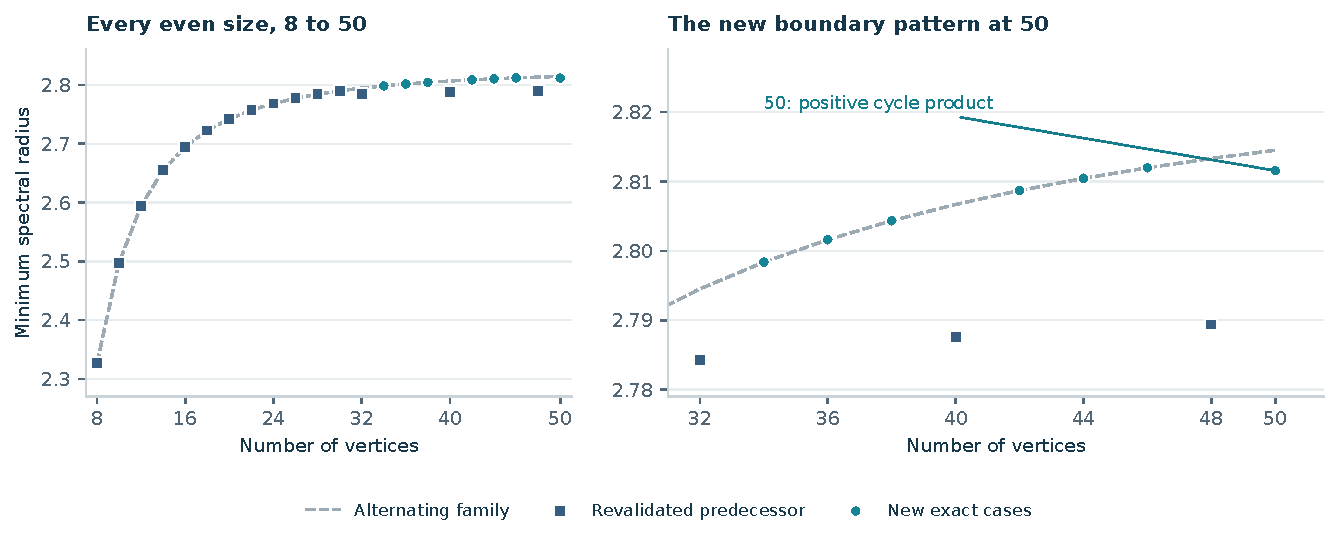
\includegraphics[width=\linewidth]{figures/cycle_optima.pdf}
\caption{Exact minimum formulas or certified values at all even sizes
through fifty. The new cases are highlighted. The thin curve is the
alternating-family value; the points at multiples of eight at least
thirty-two and at fifty fall below it. Decimal plotting is illustrative;
the proof uses exact certificates and formulas.}
\end{figure}

The next focused problem is a uniform description at lengths
\(8m+2\), \(8m+4\), and \(8m+6\). The \(50\)-vertex word is evidence for
a useful defect-pattern search, not a proof that one defect always wins.
The finite-window language can become much larger at a slightly increased
threshold, so there is additional spectral structure to analyze.

\section{A second verified transfer: density gaps}
\label{sec:density}

The incoming report \cite{IncomingDensity} addresses McNew's Questions 7.1
and 7.3 \cite{McNew}. Let \(\alpha\) be the supremum of natural densities
of sets of positive integers containing no three-term geometric
progression with rational ratio greater than one, and let
\(\overline\alpha\) use upper density. Define \(\beta,\overline\beta\)
in the same way using only integer ratios.

The verified claims are
\begin{equation}
\overline\alpha-\alpha>0.002836,\qquad
\overline\beta-\beta>0.069218.
\label{eq:density-gaps}
\end{equation}
These are existing incoming results, independently rechecked here.
They are not consequences of RH or GRH. The first strict-gap mechanism
has a short proof that makes their mathematical content assessable.

\subsection{Fixed choices versus choices varying with the cutoff}

Fix \(Y\ge12\). Let \(S\) be the positive integers with all prime factors
at most \(Y\), and put
\[
c=\prod_{p\le Y}(1-p^{-1}),\qquad
v=\prod_{p>Y}(1-p^{-2}).
\]
Write every integer uniquely as \(gh\), with \(h\in S\) and \(g\)
having no prime factor at most \(Y\). Call a set admissible if it
avoids the chosen kind of progression. Define
\[
B=c\sup_{A\subset S\text{ admissible}}\sum_{h\in A}\frac1h,\qquad
U=c\int_1^\infty J(t)\frac{dt}{t^2},
\]
where \(J(t)\) is the largest cardinality of an admissible subset of
\(S\cap[1,t]\). Since the total smooth reciprocal mass is \(1/c\),
one has \(U\le1\).

If an admissible set \(E\) has natural density \(d\), partial summation
gives
\(\sum_{n\le X,\ n\in E}1/n=(d+o(1))\log X\).
Each fixed rough fiber \(A_g=\{h:gh\in E\}\) is admissible. Hence
\[
\sum_{\substack{n\le X\\n\in E}}\frac1n
\le \frac Bc\sum_{\substack{g\le X\\g\ {\rm rough}}}\frac1g
=(B+o(1))\log X,
\]
because roughness here is a finite periodic divisibility condition.
Thus every natural density is at most \(B\).

On the other hand, squarefree rough integers have density \(cv\).
On a progression whose rough parts are squarefree, each outside prime
has three valuations in \(\{0,1\}\) in arithmetic progression, so all
three rough parts agree. This permits independent admissible choices
on each rough fiber. At cutoffs \(X_j\) with \(X_j/X_{j-1}\to\infty\),
assign each new squarefree rough \(g\in(X_{j-1},X_j]\) a maximizing
subset of \(S\cap[1,X_j/g]\), permanently. Earlier fibers can be ignored
for the lower bound at \(X_j\). For fixed \(K\), step-function summation
over \(X_j/K<g\le X_j\) gives the limiting contribution
\[
cv\int_1^K J(t)\frac{dt}{t^2}.
\]
Letting \(K\to\infty\) gives an admissible set of upper density at least
\(vU\).

The difference between \(U\) and \(B\) is strict because no one admissible
set can attain every prefix optimum. Through twelve, the greedy choice
has nine elements,
\[
\{1,2,3,5,6,7,8,10,11\},
\]
whereas
\[
\{1,2,5,6,7,8,9,10,11,12\}
\]
is admissible and has ten. The complete rational-ratio progression list
through twelve is
\[
(1,2,4),\ (1,3,9),\ (2,4,8),\ (3,6,12),\ (4,6,9);
\]
the first four have integer ratios. A set optimal at every earlier
prefix would have to agree with greedy by induction, so there is a
deficit of at least one at some integer cutoff at most twelve.
It persists throughout a unit interval and contributes at least
\(1/(12\cdot13)\) to the integral. Therefore
\[
U-B\ge \frac c{156},\qquad
u-b\ge vU-B\ge \frac c{156}-\sum_{p>Y}p^{-2},
\]
where \(u,b\) are the upper- and natural-density optima for either convention.
The Mertens product estimate and \(\sum_{n>Y}n^{-2}\le1/Y\)
give strict positivity for large \(Y\). More concretely, the exact
certificate at \(Y=2000\) gives a common gap greater than \(0.000404\).

\subsection{The stronger numbers and their scope}

The rational-ratio bound in \eqref{eq:density-gaps} uses all prefix losses
through \(80\). Its exact deficit is \(1553/45360\); the finite covering
optimization and the Euler-product tail bound were independently replayed.
For integer ratios, the certified natural-density upper bound is
\[
\beta\le\frac{5245322990569}{7001316000000}<0.749192.
\]
McNew's Theorem 4.4 gives \(\overline\beta>0.818410\) \cite{McNew}.
Their difference is greater than \(0.069218\). The incoming programs
use integer-weight branch-and-bound, not a floating optimizer.

This answers the strict comparisons posed in those questions, subject
to the written proof and finite certificates. We have not established
historical priority against every later publication. The exact value of
\(\alpha\), Rankin's optimality conjecture, and the comparison of
\(\alpha\) with \(\beta\) are not resolved by this verification.
Other attainment and computability claims in the same incoming archive
are not included in the present certificate claim.

\section{An exact Lubin--Tate coefficient window}
\label{sec:log-window}
This section advances the coefficient-depth calculation in the incoming
\emph{Cycle signings and Lubin--Tate} report.  It is a local arithmetic
method transfer, independent of RH or GRH.  The relevant source mechanism is
that a sharp integral jet bound can be attained or obstructed by isolating its
first coefficient; compare the source's
\texttt{New/Derivatives/Sharpness/OneCurve.lean}.  The new statement below is
proved directly.  We do not claim that it resolves the bounded-functions
conjecture, which separate November 2026 preprints already announce; see \cite{Colovic}.

Let $p$ be prime, let $f\ge1$ be an integer, put $q=p^f$ and $a=q-1$,
and let $L(X)\in\mathbb Q_p[[X]]$ be the
normalized Lubin--Tate logarithm with
\[
 L(X)=X+O(X^2),\qquad L(pX+X^q)=pL(X).
\]
Normalize $v_p(p)=1$.  Put $v_p(0)=+\infty$.

\begin{theorem}[Exact logarithmic coefficient window]\label{th:log-window}
For every positive integer $n$, put $N=v_p(n)$.  For every
$1\le j\le p^N$ one has
\[
 \boxed{\quad
 v_p\!\left([X^{n+j(q-1)}]L(X)^n\right)
       =N-v_p(j)-j.\quad}
\]
The coefficients outside degrees congruent to $n$ modulo $q-1$ vanish.
Consequently the first nonintegral coefficient after the leading coefficient
occurs exactly in degree
\[
 n+(q-1)J_p(N),\qquad
 J_p(N)=\min\{j\ge1:j+v_p(j)>N\}.
\]
\end{theorem}
\begin{proof}
Choose $\eta$ with $\eta^{q-1}=p$ and write
\[
 W(X)=\eta^{-1}L(\eta X)
     =X\sum_{j\ge0}\lambda_j X^{j(q-1)}.
\]
The functional equation becomes $W(pX+pX^q)=pW(X)$.
Coefficient comparison gives $\lambda_0=1$ and, for $j\ge1$,
\[
 (1-p^{j(q-1)})\lambda_j
   =\sum_{i=0}^{j-1}\lambda_i p^{i(q-1)}
         \binom{1+i(q-1)}{j-i}.
\]
Every denominator on the left is a unit.  Induction proves
$\lambda_j\in\mathbb Z_p$,
\[
 \lambda_1=(1-p^{q-1})^{-1},\qquad
 \lambda_j\in p^{q-1}\mathbb Z_p\quad(j\ge2).
\]
The support assertion follows either from the same recurrence or from the
$\mu_{q-1}$ symmetry of the functional equation.

Let $C(Y)=\sum_j\lambda_jY^j$ and $D(Y)=C(Y)-1$.  There is
$B(Y)\in Y\mathbb Z_p[[Y]]$ such that
\[
 D(Y)=\lambda_1Y(1+p^{q-1}B(Y)).
\]
For every integer $i\ge1$, all nonconstant coefficients of
$(1+p^{q-1}B)^i$ are divisible by $p^{q-1+v_p(i)}$.
Indeed
$v_p\binom{i}{k}\ge v_p(i)-v_p(k)$ and
$(q-1)k-v_p(k)\ge q-1$ for $k\ge1$.
It follows that for $j>i$,
\[
 v_p([Y^j]D(Y)^i)\ge q-1+v_p(i).
\]
Expand $C^n=\sum_i\binom niD^i$.  For $1\le j\le p^N\le n$,
the term $i=j$ has coefficient $\binom nj\lambda_1^j$.  Its valuation is
$N-v_p(j)$: use
$\binom nj=(n/j)\binom{n-1}{j-1}$ and note that the last binomial is a
$p$-adic unit since the lowest $N$ base-$p$ digits of $n-1$ are all $p-1$.
Every term $i<j$ has valuation at least $N+q-1$, by the preceding inequality
and $v_p\binom ni\ge N-v_p(i)$.  Thus no cancellation is possible and
\[
 v_p([Y^j]C^n)=N-v_p(j).
\]
Since $[X^{n+ja}]W^n=p^j[X^{n+ja}]L^n$, the asserted equality follows.
Finally $J_p(N)\le N+1\le p^N$ (also when $N=0$), so the proven range includes
the first failure of integrality.
\end{proof}

The case $p=q=2$ gives $L(X)=\log(1+X)$; the theorem then recovers an
exact coefficient-valuation formula for powers of the usual formal
logarithm.  The proof above uses only $q-1\ge1$, so the stated uniformity
in the residue degree requires no additional hypothesis.

For computation, the threshold also has the closed finite expression
\[
 J_p(N)=\min_{0\le b\le\lfloor\log_p(N+1)\rfloor}
 p^b\left(\left\lfloor\frac{N-b}{p^b}\right\rfloor+1\right).
\]
To see this, the expression for a fixed $b$ is the first positive multiple
of $p^b$ whose sum with $b$ exceeds $N$.  It always satisfies the required
inequality, and every minimizing $j$ is included by taking $b=v_p(j)$.

\subsection{Consequence for the genuine coefficient-depth invariant}
For this application specialize again to $q=p^2$.  Let $K/\mathbb Q_p$
be unramified quadratic, let
$M=\mathcal O_K[[X]]^{\psi=0}$, and write
\[
 f([T](X))=\sum_{m\ge0}c_{f,m}(T)X^m.
\]
Berger--Sprang's $s_0(n)$ is the least $m\ge n$ for which the
$\mathcal O_K$-span of the $c_{f,r}$ with $r\le m$ contains a polynomial of
\emph{degree $n$} and leading coefficient of valuation $-w_q(n)$, where
$w_q(n)=\sum_{r\ge1}\lfloor n/q^r\rfloor$.

\begin{corollary}[A sharp coefficient obstruction]\label{cor:depth-window}
Let $n>0$. If $s_0(n)>n$, then
\[
 s_0(n)\ \ge\ n+(q-1)J_p(v_p(n)).
\]
\end{corollary}
\begin{proof}
Write $E=L^{-1}$.  The coefficient identity
\[
 [T^n]c_{f,m}(T)=[Z^n]f(E(Z))\,[X^m]L(X)^n
\]
follows by substituting $[T](X)=E(TL(X))$.
At $m=n$, the second factor is one.  Since each $c_{f,n}$ is integer-valued
and has degree at most $n$, its leading coefficient has valuation at least
$-w_q(n)$.  Failure at depth $n$, and the integral value group of $K$, imply
that every first factor has valuation at least $1-w_q(n)$.  The theorem
shows that all second factors before the indicated threshold are integral.
Thus all $T^n$ coefficients in the entire generated module have valuation
at least $1-w_q(n)$, which excludes the required degree-$n$ polynomial.
\end{proof}

The equality in Theorem~\ref{th:log-window} resolves the precise first
integrality threshold which the earlier report bounded using
$j+\lfloor\log_pj\rfloor$.  It does \emph{not} prove that $s_0(n)$ equals the
new lower bound.  At later depths a $T^n$ coefficient of the right valuation
may occur in a polynomial of higher degree.  Those higher terms must be
eliminated by integral combinations of genuine trace-kernel rows.  This
is a distinct arithmetic constraint.

\subsection{A necessary correction to the numerical baseline}
Berger's primary-source errata, dated 13 October 2026, identifies an error in
the paper's Appendix A implementation: at each stage it inserts $T^s$
without establishing membership in the module and omits the genuine
possible nonunit diagonal generator.  Consequently its printed experiment
addresses $\operatorname{Pol}(M)+\mathcal O_K[T]$ rather than the defined
$s_0(n)$.  The theoretical definition and the trace-kernel generators remain
usable.  The incoming report's independent proof of the small-digit-sum
criterion is not invalidated by this code error.

The accompanying \texttt{coefficient\_depth.py} starts only from the exact
trace-kernel generators
\[
 X^i(pX+X^q)^j\quad(1\le i\le q-2),\qquad
 (pX^{q-1}+q-1)(pX+X^q)^j.
\]
It forms the logarithm's Carleman matrix $D$, inverts it over the rational
numbers, and forms genuine rows using $D^{-1}\operatorname{diag}(1,T,\dots)D$.
For a cutoff $N$, it suffices to use $j\le N$ in the second family and
$i+j\le N$ in the first: the omitted generators have $X$-adic order
greater than $N$, since $pX+X^q$ has $X$-adic order one.  Every trace-kernel
series is a convergent $\mathcal O_K$-linear combination of these generator
series, and its coefficients through $X^N$ depend only on the finite list.
All rows $c_{f,m}$ with $m\le N$ are retained, including diagonal rows with
nonunit coefficients.  This proves completeness at each finite cutoff.

A descending-degree elimination over $\mathbb Z_{(p)}$ replaces a pivot only
when a smaller valuation is found.  Every row operation is invertible over
that ring.  An echelon row of leading degree $n$ therefore gives exactly the
leading-coefficient ideal of the intersection with polynomials of degree
at most $n$.  Extension to $\mathcal O_K$ preserves this calculation.
No finite $p$-adic precision or added monomial is used.

An independent integer Hermite-normal-form calculation confirms the following
exact values.  The two valuation columns give the leading-coefficient ideal
for degree $n$ after imposing that all higher-degree terms vanish.
\begin{center}
\begin{tabular}{rrrrrr}
$p$ & $q$ & $n$ & $s_0(n)$ & valuation at $s_0(n)-1$ & valuation at $s_0(n)$\\
\hline
2&4&3&6&1&0\\
2&4&5&8&0&-1\\
2&4&7&16&0&-1\\
2&4&12&30&-2&-3\\
3&9&8&16&1&0
\end{tabular}
\end{center}
For $p=2,n=12$, Theorem~\ref{th:log-window} first allows a suitable
$T^{12}$ coefficient in a row at depth $18$, since $v_2(12)=2$ and
$J_2(2)=2$.  The exact module calculation gives $s_0(12)=30$.
Indeed, the genuine generator $g(X)=2X^3+3$ already gives
$[T^{12}]c_{g,18}(T)=15811/9815288$, of valuation $-3$.
Thus reaching the right coefficient valuation alone is insufficient;
eliminating all higher terms can require additional rows.

For the independent check, clear denominators in each rational row using
only $p$-adic units and a common factor $p^K$.  Choose a triangular full-rank
source submatrix whose determinant has valuation $M$.  Its adjugate proves
that $p^M\mathbb Z_p^d$ is already in the scaled row module.  Adding $p^M I$
and reducing entries modulo $p^M$ therefore preserves that module.  Exact
integer column Hermite normal form now gives its leading-degree ideals;
subtracting $K$ restores the original valuations.  The script
\texttt{verify\_depth\_hnf.py} records both the obstruction immediately
before each claimed depth and attainment at that depth.  Monotonicity of
the generated modules proves that these are exact minima, rather than
upper bounds from finding one witness.

The attached JSON files record exact finite computations; a null entry
means only that the cutoff was exceeded.  The finite-ring script
\texttt{verify\_log\_window.py} independently checks the displayed universal
valuation formula for several primes and ranges.  These are reproducible
arithmetic checks supporting the written proof, not Lean kernel checks.

\paragraph{Sources and novelty boundary.}
The primary inputs are \cite{BS,BergerErrata}, namely Berger--Sprang, \emph{Integer-valued polynomials and
$p$-adic Fourier theory}, arXiv:2502.18053, Definition 5.1 and Lemma 5.2;
Berger, \emph{Errata for my articles}, Section 19,
\url{https://perso.ens-lyon.fr/laurent.berger/articles/errata.pdf}; and the
incoming \emph{Cycle signings and Lubin--Tate} manuscript, Section
\emph{When is the first coefficient depth sufficient?}.  The exact
coefficient formula and corrected computation here are new to the reviewed
incoming corpus.  No claim of exhaustive literature priority is made.

% Standalone input section; requires amsmath, amssymb, amsthm in parent document.
\Needspace{10\baselineskip}
\section{A finite certificate for the conjugate-dual congruence term}
\label{sec:congruence-smith}

The following is elementary linear algebra over a discrete valuation ring. Its
value here is diagnostic: it identifies exactly when a hypothesis of the
upstream twisting theorem can hold, and provides a finite certificate when it
does. The structural incoming report already uses this viewpoint
\cite{IncomingStructural}; we make no claim of historical novelty for the
linear algebra.

Let $O$ be a discrete valuation ring with uniformizer $\pi$ and fraction field
$K$. Let $T,U$ be finite free $O$-modules with actions of a group $G$. Put
$V=\operatorname{Hom}_O(T,U)$, of rank $m$, and let $R\subseteq V^*$ be the
$O$-submodule generated by all coordinate equations of
\[
 \rho_U(g)f-f\rho_T(g)=0\qquad(g\in G).
\]
Write
\[
 Q:=V^*/R\simeq O^d\oplus\bigoplus_i O/(\pi^{a_i}),\qquad a_i>0.
\]
Then for every $k\geq1$ there is an $O$-linear identification
\[
 \operatorname{Hom}_G(T/\pi^kT,U/\pi^kU)
 \simeq\operatorname{Hom}_O(Q,O/\pi^k),
\]
and consequently the exact formula
\begin{equation}
 \operatorname{length}_O\operatorname{Hom}_G(T/\pi^kT,U/\pi^kU)
   =dk+\sum_i\min(k,a_i).
 \label{eq:congruence-smith-length}
\end{equation}

Indeed, a vector of $V/\pi^kV$ is a functional on $V^*$ with values in
$O/\pi^k$; equivariance says exactly that it annihilates $R$. A free summand
of $Q$ contributes length $k$, whereas $O/\pi^a$ contributes the
$\pi^a$-torsion in $O/\pi^k$, of length $\min(a,k)$. Furthermore,
\[
 d=\dim_K\operatorname{Hom}_G(T\otimes_OK,U\otimes_OK).
\]
It follows that the supremum of the left-hand side of
\eqref{eq:congruence-smith-length} is finite if and only if this rational Hom
space is zero. In that case the supremum is $\sum_i a_i$, reached for
$k\geq\max_i a_i$ when torsion factors are present, and immediately if
there are none. Nonzero ideals of a DVR are powers of its maximal ideal,
so the same conclusion holds for the supremum over arbitrary $a\in O\setminus\{0\}$.

\paragraph{Finite certificates and their limitation.}
Noetherianity implies that finitely many of the original coordinate equations
generate $R$. Finding such a complete set effectively is a separate issue.
There is, however, a useful sufficient certificate: choose any finite relation
matrix $M$ of full column rank $m$. If its Smith exponents are
$b_1,\ldots,b_m\geq0$, the true equivariant Hom is a submodule of the kernel
of $M$ modulo $\pi^k$, whence
\[
 \operatorname{length}_O\operatorname{Hom}_G(T/\pi^kT,U/\pi^kU)
 \leq\sum_{i=1}^m\min(k,b_i)\leq\sum_{i=1}^m b_i.
\]
Any nonzero maximal minor $\Delta$ gives the coarser bound
$\sum b_i\leq v_\pi(\Delta)$. Thus a finite sample can certify an upper
bound without a claim that it generates all Galois relations. It cannot by
itself certify that a nonzero kernel persists after the omitted relations.

\paragraph{Exact correspondence with \texttt{grh-lean}.}
Here take $O$ to be the integer ring of a finite extension of
$\mathbb Q_\ell$, as in the source interface.
In \texttt{New.Selmer.conjDualHom}, take $G=\operatorname{Gal}(\Omega/E)$,
$T=O^n$, $A_g=\rho(g)$, $c(g)=\texttt{conjGal}(g)$, and let $\chi$ denote
the $\ell$-adic cyclotomic character. The source equation for $\eta$ is
\[
 \eta(A_g u)(v)=\eta(u)\bigl(\chi(c(g))A_{c(g)^{-1}}v\bigr).
\]
The source's \texttt{CharacterModule} is the additive character dual with
values in $\mathbb Q/\mathbb Z$. Since the trace-dual lattice
$O^\vee=\operatorname{Hom}_{\mathbb Z_\ell}(O,\mathbb Z_\ell)$ is an
invertible, hence free rank-one, $O$-module, choosing a generator identifies
$a^{-1}O^\vee/O^\vee$ with $O/a$. Thus $\eta$ is represented, noncanonically,
by a balanced bilinear pairing matrix $B$ modulo $a$. Its relations are
exactly
\begin{equation}
 A_g^{\mathsf T}B A_{c(g)}-\chi(g)B=0\pmod a,
 \label{eq:conj-dual-relations}
\end{equation}
using $\chi(c(g))=\chi(g)$. The relation module therefore has $m=n^2$.
Its rational kernel is
$\operatorname{Hom}_G(T_K,T_K^{\vee,c}(1))$.
Accordingly, the upstream \texttt{congruenceTerm} is finite precisely when
this rational Hom vanishes, and then its value is the sum of the Smith
exponents of all the relations. This concerns only the representation term;
it does not identify the upstream cocycle model with a standard Selmer group.

\paragraph{Ramification.}
Let $O'/O$ have relative ramification index $e$ and transport the \emph{same}
representations by scalar extension. Flatness gives $Q'=Q\otimes_OO'$;
the free rank remains $d$ and the elementary exponents become $ea_i$.
Hence the length at $\pi'^k$ is $dk+\sum_i\min(k,ea_i)$.
If $e_0=v_\pi(\ell)$, the normalization in the source divides $O$-length by
$e_0$ and $O'$-length by $ee_0$. The finite normalized supremum is invariant:
\[
 \frac{e\sum_i a_i}{ee_0}=\frac{\sum_i a_i}{e_0}.
\]
At corresponding moduli $\pi^k$ and $\pi'^{ek}$, normalized lengths agree
term by term. Coefficient extension alone cannot remove a rational
conjugate-dual obstruction.

This does not license a vanishing argument for \emph{varying} twists and
coefficient fields. The nonzero module $O'/\pi'$ has normalized length
$1/(ee_0)$, tending to zero as $e$ grows. A fixed-ring bound strictly below
$1/e_0$ forces vanishing, but a bound with the ring and twist depending on
the error tolerance does not. This quantifier distinction is required when
using \texttt{exists\_anticyclotomic\_twist}.

\paragraph{Exact examples and reproducibility.}
The accompanying checker uses only Python's standard library. It obtains
integer Smith factors from gcds of all minors and independently enumerates
small modular kernels. For a rank-one relation $5^a f=0$ over $\mathbb Z_5$,
the length is $\min(k,a)$; for the zero relation it is $k$. Thus residual
isomorphism alone is not the obstruction: rational equivariant Hom is.
For the abstract cyclic example $A=C=\operatorname{diag}(1,26)$,
$\chi=126$, relation~\eqref{eq:conj-dual-relations} has $5$-adic Smith
exponents $(2,2,2,3)$ and supremum $9$. Restriction to symmetric and
alternating matrices gives exponents $(2,2,3)$ and $(2)$, respectively.
These are illustrative matrix certificates, not arithmetic Galois-image
certificates. In residue characteristic two, an alternating constraint must
include zero diagonal entries in addition to off-diagonal skew symmetry.

\Needspace{12\baselineskip}
\section{What this means for other arithmetic conjectures}
\label{sec:targets}

The new certified examples establish that the repository and incoming work
are useful sources of methods. They do not reduce every open problem to
matrix manipulation. The following targets have different remaining
mathematical requirements.

\subsection{A concrete nonabelian benchmark}

Let \(F=\Q(\theta)\), where \(\theta^3-\theta-1=0\). The cubic has no
rational root and has discriminant \(-23\), so its normal closure has
Galois group \(S_3\). The cubic permutation representation decomposes as
\(\mathbf1\oplus\rho\), where \(\rho\) has dimension two; the Artin
factorization is
\[
\zeta_F(s)=\zeta(s)L(s,\rho).
\]
For unramified primes, \(\operatorname{tr}\rho(\mathrm{Frob}_p)\) is the
number of roots of \(X^3-X-1\) modulo \(p\), minus one.
The identity, transposition, and three-cycle values are \(2,0,-1\).
This information is not determined by a fixed abelian congruence class.

The preceding nonabelian reports isolate one-sided prime estimates
and more elaborate nonnegative detectors for this and related fields
\cite{IncomingNonabelian,IncomingBridges}. A transparent statistic is
the smoothed Dedekind prime-ideal sum
\[
S_F(x)=\sum_{N\mathfrak p^k\le x}
\log N\mathfrak p
\left(\frac1{N\mathfrak p^k}-\frac1x\right).
\]
Its principal main term is \(\log x+c_F\).
An appropriate eventual upper estimate of
\(S_F(x)-\log x-c_F\) at square-root quality, together with the
analytic sign conditions, would give a new zero-location result.
The unresolved arithmetic task is to make the source's integral
construction record these splitting types and retain all required
uniform size, spanning, and determinant bounds.

The earlier discriminant-\(229\) analysis is useful: it identifies
an integral-frame obstruction and a possible projective-lattice remedy.
Those are local advances. Their existence alone does not imply the
needed global estimate. A sensible next milestone is one explicitly
stated uniform inequality for one fixed cubic field.

\subsection{Algebraic \texorpdfstring{\(K\)}{K}-theory and Selmer problems}

The source's cyclotomic odd-cocycle bound supplies a uniform arithmetic
integer controlling lengths. It is a promising input to finite
vanishing certificates. However,
\src{Lib/Cyclotomic/OddSha.lean}{\texttt{OddSha.lean}} explicitly separates
its cocycle model from a comparison with standard \(\Sha^1\), and does
not prove an equality of Iwasawa characteristic ideals.

To turn this into a \(K\)-group computation, one needs a correct
comparison with the relevant cohomology or Selmer group, all local
conditions and parity conventions, and the finite arithmetic certificate
in the right order of quantifiers. An abstract small length is insufficient.
The congruence diagnostic in Section~\ref{sec:congruence-smith} gives a
quick preliminary screen: rational conjugate self-duality makes the
full congruence term infinite. When that obstruction is absent,
actual full-rank relation minors can certify a finite bound.

The question is whether the arithmetic data satisfy the source theorem's
hypotheses. A matrix example with the same shape is not enough.
Accordingly, no Vandiver, general \(K_{4m}(\Z)\)-vanishing, or BSD
conclusion is asserted here.

\subsection{Why direct elliptic-curve or BSD transplantation fails}

The source \code{SelmerDatum} requires absolute residual irreducibility,
finite global and local terms, specified inertia behavior, and compatibility
of a conjugate-dual pairing with the mirror construction.
An elliptic Tate module is polarized, and its inertia and pairing data
cannot simply be substituted into an interface designed for the source's
special representations.

The previous structural report already discusses the pairing-sign
obstruction \cite{IncomingStructural}. The exact Smith-factor viewpoint
adds an operational test of finiteness, but does not remove that
obstruction. A successful application would need a theorem about
the correct signed or quotiented component and its actual local
conditions, followed by a comparison to the desired arithmetic group.

\subsection{Zero simplicity and correlations}

The endgame locates zeros by excluding poles of transforms with controlled
signs. It does not distinguish a zero of multiplicity one from a zero
of larger positive multiplicity on the allowed line. Nor do coarse
one-sided prime estimates encode pair correlation at microscopic
scales. Transferring the zero-location conclusion to simplicity,
linear independence of ordinates, or random-matrix statistics would
require new observables and estimates.

\subsection{Research priorities after this report}

\begin{center}
\begin{tabularx}{\linewidth}{@{}p{0.24\linewidth}X@{}}
\toprule
\textbf{Next problem} & \textbf{A concrete success criterion}\\
\midrule
Other cycle lengths &
Classify the allowed defect patterns and prove exact optima for an
infinite residue class outside \(8\Z\). The new \(50\)-vertex certificate
is a test case with positive holonomy.\\
Coefficient-depth growth &
Prove matching upper bounds on delayed \(s_0(n)\) using genuine
trace-kernel rows and integral elimination. The exact coefficient
threshold does not by itself control higher-term cancellation.\\
Fixed nonabelian field &
Prove a Frobenius-sensitive arithmetic inequality with constants and
uniformity sufficient for the analytic detector.\\
Finite arithmetic vanishing &
Complete the standard-Selmer comparison and supply the necessary
arithmetic determinant or Hecke certificate, with explicit coefficient rings.\\
\bottomrule
\end{tabularx}
\end{center}

\Needspace{24\baselineskip}
\section{Reproduction and formalization boundaries}
\label{sec:reproduction}

The decisive computations can be rerun without network access.
Python's standard library suffices for the new graph proofs, the modular
coefficient-window checks, the main coefficient-module calculation, and the
congruence examples. The independent integer Hermite-normal-form check
uses SymPy. Plot regeneration uses Matplotlib.
The PDF source compiles with ordinary pdfLaTeX.

\begin{center}
\begin{tabularx}{\linewidth}{@{}p{0.38\linewidth}X@{}}
\toprule
\textbf{Location} & \textbf{Contents}\\
\midrule
\code{report.tex}, \code{sections/} & Complete manuscript, including proofs.\\
\code{checks/graphs/} & Six-case exact verifier and its output.\\
\code{checks/graphs/n50/} & Two independent exact verifiers, full survivors,
integer characteristic polynomial, and certified root interval.\\
\code{checks/local/} & General coefficient-window checks; corrected
coefficient-depth algorithm; independent HNF checks and tables.\\
\code{checks/congruence/} & Smith-factor examples and brute modular checks.\\
\code{checks/predecessors/} & Inspected predecessor programs and replay logs
for the graph and density results.\\
\code{provenance/} & Pinned revisions, 46-archive inventory, source hashes,
verification scope, and commands.\\
\code{sources/} & Selected unmodified upstream files with notices, and
the relevant predecessor evidence sections.\\
\bottomrule
\end{tabularx}
\end{center}

The main certificate commands are listed in \code{README.txt}.
They generate the same mathematical data regardless of decimal plotting
precision. A \code{null} coefficient-depth entry in a JSON table means
only that the specified finite cutoff was exceeded.

The new graph proof can be formalized by defining the signed graph,
proving the switching classification and compression inequality,
checking the finite positive-definiteness certificates, and then proving
the trigonometric or polynomial description of the winning spectrum.
The finite lists could be verified in Lean by a small exact arithmetic
checker; the present Python computation is not that formal proof.

The local-series proof requires coefficient recurrences, the valuation
of binomial coefficients in the initial \(p\)-adic digit window, and the
unique term of lowest valuation. It does not depend on the complete
upstream GRH development. The coefficient-depth computations need an
additional verified theorem that the finite row list spans the truncated
trace-kernel coefficient module, followed by a verified lattice
elimination algorithm.

The source inspection, exact computations, and written arguments support
the specific claims made above. They do not constitute a blanket
verification of the 46 earlier archives or of every intended use of
the source's custom foundational interfaces.

\clearpage
\begin{thebibliography}{99}
\small
\raggedright
\bibitem{Repo}
The \texttt{lsernau/grh-lean} contributors.
\emph{GRH for Dirichlet \(L\)-functions, in Lean 4}.
Revision \texttt{72fead102f663d5c7a407964a13dc0cf9d977207}.
\url{https://github.com/lsernau/grh-lean}.
Proof attributed there to Levent Alp\"oge with Claude; shortened development
credited to Anthropic collaborators and Claude.

\bibitem{Incoming}
Vladimir Reshetnikov, \emph{ProveIt: incoming research reports}.
Revision \texttt{5cc267af75a635199ac5d93a7d49cbce521daefc}.
\url{https://github.com/VladimirReshetnikov/ProveIt/tree/5cc267af75a635199ac5d93a7d49cbce521daefc/docs/incoming}.
Full archive inventory and hashes accompany this report.

\bibitem{IncomingCycle}
\emph{Optimal signings of square cycles and sharp Lubin--Tate jet recovery},
25 November 2026, in \cite{Incoming},
\nolinkurl{grh_transfers_cycle_signings_and_lubin_tate.zip}.
The graph portion was independently replayed; the local portion is
extended and its computational context corrected here.

\bibitem{IncomingDensity}
\emph{Density gaps and zero tests}, in \cite{Incoming},
\nolinkurl{grh_transfers_density_gaps_and_zero_tests.zip}.
Sections \emph{Two density questions of McNew over the integers} and
\emph{A larger separation from the first eighty integers}.

\bibitem{IncomingNonabelian}
\emph{Nonabelian transfer report}, in \cite{Incoming},
\nolinkurl{grh_nonabelian_transfer_2026-11-25.zip}.
Used for its stated nonabelian interfaces and open obligations;
the whole arithmetic program is not certified here.

\bibitem{IncomingBridges}
\emph{Transfer bridges}, in \cite{Incoming},
\nolinkurl{grh_transfer_bridges_2026-11-25.zip}.

\bibitem{IncomingStructural}
\emph{Structural transfers}, in \cite{Incoming},
\nolinkurl{grh_structural_transfers_2026-11-25.zip}.
Contains the earlier congruence-length and polarization obstruction.

\bibitem{Suvagiya}
Vaibhav Suvagiya.
\emph{Parity families and signed spectra: kernel averaging,
near-Ramanujan bounds, and exact circulant models}.
arXiv:2607.17343v2, 22 September 2026.
\url{https://arxiv.org/html/2607.17343v2}.
Especially Proposition 25, Theorem 26, Conjecture 28, and Remark 29.

\bibitem{Trure}
trureturing.
\emph{Suvagiya Conjecture 28 refutation}.
\url{https://www.trureturing.org/research/suvagiya-conjecture28-refutation/}.
The prior \(32\)-vertex counterexample is distinct from a proof of the
unrestricted exact optimum.

\bibitem{McNew}
Nathan McNew.
On sets of integers which contain no three terms in geometric progression.
\emph{Mathematics of Computation} \textbf{84} (2015), 2893--2910.
\url{https://www.nathanmcnew.com/GPFsets.pdf}.
Especially Theorem 4.4 and Questions 7.1--7.4.

\bibitem{BS}
Laurent Berger and Johannes Sprang.
\emph{Integer-valued polynomials and \(p\)-adic Fourier theory}.
arXiv:2502.18053v2, 2025.
\url{https://arxiv.org/abs/2502.18053}.
Definition 5.1 and Lemma 5.2; the Appendix A code must be read
together with \cite{BergerErrata}.

\bibitem{BergerErrata}
Laurent Berger.
\emph{Errata for my articles}, dated 13 October 2026, Section 19.
\url{https://perso.ens-lyon.fr/laurent.berger/articles/errata.pdf}.

\bibitem{Colovic}
Uro\v{s} A. Colovi\'c.
\emph{On the ring of bounded functions on the character variety}.
arXiv:2611.25162v1, 18 November 2026.
\url{https://arxiv.org/abs/2611.25162}.
Its announced qualitative result is separate from the quantitative
coefficient-depth problem studied here.
\end{thebibliography}

\end{document}
